\begin{question}[section=1,name={15.06.2016},mode=exm,type=bsp,tags={20160615}]
	Eine dreisträngige symetrisch aufgebaute 4-polige (p=2) permanentmagneterregte Synchronmaschine in Y-Schaltung mit $I_N = 15~A$ (Effektivwert) und $n_N= 1500~U/min$ habe zu dem betrachteten Zeitpunkt $\tau_0$ einen normierten Rotorverkettungsfluss von $\underline{\Psi}_M = 1 \cdot e^{-\jmath 20 ^\circ}$. Zu diesem Zeitpunkt $\tau_0$ ist der normierte statorfeste Stromraumzeiger $\underline{i}_s = -0,15 -\jmath0,9$.
	\begin{compactenum}
		\item Berechnen Sie für diesen Zeitpunkt $\tau_0$ die bezogenen Strangströme $i_1$, $i_2$ und $i_3$ sowie die nicht bezogenen Ströme $I_1$, $I_2$ und $I_3$. (\addpoints{2})
		\item Berechnen Sie für den Zeitpunkt $\tau_0$ den normierten Stromraumzeiger im rotorfesten Koordinatensystem und das bezogene Drehmoment der Maschine. Skizzieren Sie die Raumzeiger $\underline{\Psi}_M$ und $\underline{i}_s$ sowie die dem Moment entsprechende Fläche in der komplexen Raumzeigerebene (Strangachse ``U'' liegt in der reellen Achse) des obrigen Betriebpunktes. (\addpoints{2})
		\item Berechnen Sie alternativ für den BLDC-Betrieb zum Zeitpunkt $\tau_0$ jenen normierten Stromraumzeiger im statorfesten Koordinatensystem, welcher das \textbf{generatorische} Bezugsmoment bei positiver Drehrichtung ergibt. (Die Berechnung soll unter optimaler Drehmomentenausbeute erfolgen). Geben Sie ebenfalls die d- und q- Stromkomponenten für diesen an. (\addpoints{3}) \label{20160615Bsp1}
		\item Skizzieren Sie die Raumzeiger $\underline{\Psi}_M$ und $\underline{i}_s$ sowie die dem Moment entsprechende Fläche in der komplexen Raumzeigerebene (Strangachse ``U'' liegt in der reellen Achse) des obrigen BLDC-Betriebpunktes. (\addpoints{1})
		\item Skizzieren Sie den Zeitverlauf des nicht bezogenen Strangstroms $I_1(t)$ [$A$] in Abhängigkeit der Zeit $t$ [$ms$] ab dem Zeitpunkt $t_0$ ensprechend Frage \ref{20160615Bsp1}.) für den BLDC-Betrieb, wenn die PSM mit einer positiven Drehzahl von $\omega_m = 0,1$ bei \textbf{konstantem generatorischem Bezugsmoment} läuft. (\addpoints{2})
	\end{compactenum}
\end{question}
\begin{solution}
	\begin{compactenum}
		\item Da zum Zeitpunkt $\tau_0$ der Rotorverkettungsfluss dem Stromraumzeiger voreilt, kann es sich in diesem Beispiel nur um ein linksdrehenden Generator oder um einen rechtsdrehenden Motor handeln. Zuerst wird der Statorstrom in Polarkoordinaten gebracht.
		\begin{align}
			|\underline{i}_s|  &= \sqrt{0,15^2 + 0,9^2}= 0,912 \\
			\arg(\underline{i}_s) & =-90 - \arctan\left (\frac{0,15}{0,9} \right ) =-99,46 \\
			\underline{i}_s  &= 0,912 \cdot e^{-\jmath 99,46 ^\circ}
		\end{align}
		In die Glg.(\ref{glg:strang1}),(\ref{glg:strang2}) und (\ref{glg:strang3}) wird der Statorstrom $\underline{i}_s$ eingesetzt.
		\begin{align}
			i_1 & = \Re \{ \underline{i}_s \cdot e^{\jmath \cdot 0 ^\circ} \} = -0,15\\
			i_2 & = \Re \{ \underline{i}_s \cdot e^{-\jmath \cdot 120 ^\circ} \} = -0,709 \\
			i_3 & = \Re \{ \underline{i}_s \cdot e^{\jmath \cdot 120 ^\circ} \}=  0,851
		\end{align}
		Um die nicht bezogenen Ströme zu erhalten werden die bezogenen Ströme mit dem Bezugswert $I_N \cdot \sqrt{2}$ multipliziert. (Effektivwert auf Spitzenwert umrechnen)
		\begin{align}
			I_1 & = i_1 \cdot I_N \cdot \sqrt{2} = -0,15 \cdot 15 A \cdot \sqrt{2} =-3,18~A \\
			I_2 & = i_2 \cdot I_N \cdot \sqrt{2} = -0,709 \cdot 15 A \cdot \sqrt{2} = -15,04~A\\
			I_3 & = i_3 \cdot I_N \cdot \sqrt{2} = 0,851\cdot 15 A \cdot \sqrt{2} =18,05~A
		\end{align}
		\item Im Rotorfesten Koordinatensystem ist der Stromzeiger um $20^\circ$ in positiver Drehrichtung verschoben. Der Statorstrom wird auch gleich in seine komponenten $\underline{i}_{sq}$ und $\underline{i}_{sd}$ aufgeteilt. Dann wird $\underline{i}_{sq}$ und $\Psi_M$ in Glg.(\ref{glg:synmoment}) eingesetzt.
		\begin{align}
			\underline{i}_{sdq} & = \underline{i}_s \cdot e^{\jmath 20 ^\circ} = 0,912 \cdot e^{-\jmath 99,46 ^\circ} \cdot e^{\jmath 20 ^\circ} = 0,912 \cdot e^{-\jmath 79,46 ^\circ} \\
			\underline{i}_{sd} & = |\underline{i}_{sdq}| \cdot \cos(\arg(\underline{i}_{sdq})) = 0,912 \cdot \cos(-79,46) = 0,166 \\
			\underline{i}_{sq} & = |\underline{i}_{sdq}| \cdot \sin(\arg(\underline{i}_{sdq})) = 0,912 \cdot \sin(-79,46) = -0,896 \\
			m_R(\tau)& =  i_{sq} \cdot | \underline{\Psi}_M|= -0,896 \cdot 1 = -0,896
		\end{align}
		Da das Moment negativ ist, ist hier ersichtlich, dass es sich um einen generatorischen linksbetrieb handelt.
		\begin{figure}[H]
			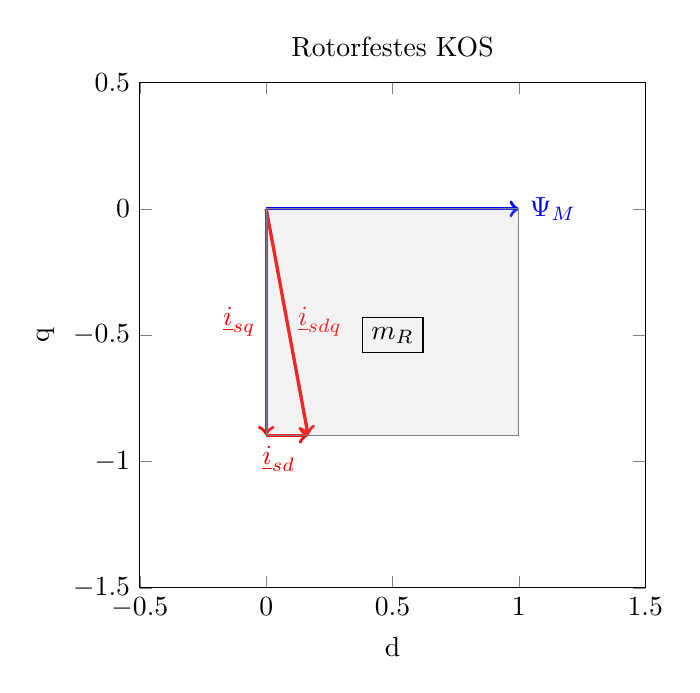
\begin{tikzpicture}
				\begin{axis}[title={Rotorfestes KOS},xlabel={d}, ylabel={q},
					xtick= {-.5,0,...,1.5},width=8cm,height=8cm,
					xmin = -.5,xmax = 1.5,
					ytick= {-1.5,-1,...,0.5},
					ymin = -1.5 , ymax = .5]
					\addplot [->,blue,no marks,very thick ]coordinates { (0,0) (1,0)}node[pos=1,anchor=west]{$\Psi_M$}; % Psi_m
					\addplot [->,red,no marks,very thick]coordinates { (0,0) (0,-0.896)}node[pos=0.5,anchor=east]{$\underline{i}_{sq}$};
					\addplot [->,red,no marks,very thick]coordinates {(0,-0.896) (0.166 , -0.896)}node[pos=0.3,anchor=north]{$\underline{i}_{sd}$};
					\addplot [->,red,no marks,very thick]coordinates { (0,0) (0.166,-0.896)}node[pos=0.5,anchor=west]{$\underline{i}_{sdq}$};
					\addplot [const plot, fill=gray!50,fill opacity=0.2, draw=black!50] coordinates {
						(0, 0) (0,-0.896) (1,-0.896) (1,0)}\closedcycle;
					\node[draw=black] at (axis cs:0.5,-0.5) {$m_R$};
				\end{axis}
			\end{tikzpicture}
			\label{fig:20160615lsg12}
		\end{figure}
		\item Der optimalste Stromvektor steht normal auf den Rotorverkettungsfluss. Der nächstgelegene Stromraumzeiger zu $e^{-\jmath 110 ^\circ}$ ist Fall F bei $-90 ^\circ$. Generatorisches Bezugsmoment heißt, dass $m_R=-1$ sein muss. Optimale Drehmomentausbeute bedeutet, dass $\underline{i}_{sq} = -1$ sein muss. (Negativ weil generatorisch)
		\begin{align}
			m_{R,BLDC}(\tau)& =  i_{sq} \cdot | \underline{\Psi}_M|\\
			\arg(\underline{i}_{sdq}) &= \arg(\underline{i}_s) - \arg(\underline{\Psi}_M) = -90 - (-20) = -70^\circ \\
			|\underline{i}_{sdq}| &= \frac{i_{sq}}{\sin(\arg(\underline{i}_{sdq}))}= \frac{-1}{-0,939}=1,064 \\
			\underline{i}_{sd} & = |\underline{i}_{sdq}| \cdot \cos(\arg(\underline{i}_{sdq}))=1,064 \cdot \cos(-70)=0,363
		\end{align}
		\item 
		\begin{figure}[H]
			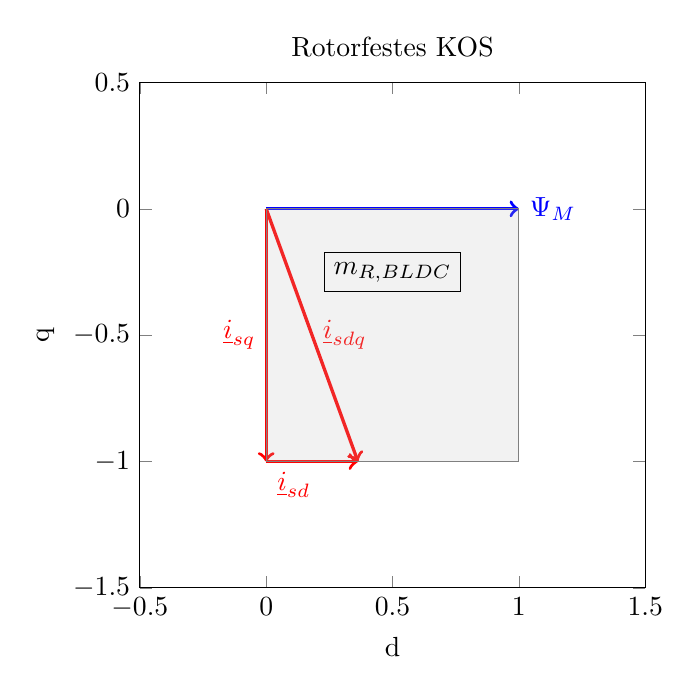
\begin{tikzpicture}
				\begin{axis}[title={Rotorfestes KOS},xlabel={d}, ylabel={q},
					xtick= {-.5,0,...,1.5},width=8cm,height=8cm,
					xmin = -.5,xmax = 1.5,
					ytick= {-1.5,-1,...,0.5},
					ymin = -1.5 , ymax = .5]
					\addplot [->,blue,no marks,very thick ]coordinates { (0,0) (1,0)}node[pos=1,anchor=west]{$\Psi_M$}; % Psi_m
					\addplot [->,red,no marks,very thick ]coordinates { (0,0) (0,-1)}node[pos=0.5,anchor=east]{$\underline{i}_{sq}$};
					\addplot [->,red,no marks,very thick ]coordinates {(0,-1) (0.363 , -1)}node[pos=0.3,anchor=north]{$\underline{i}_{sd}$};
					\addplot [->,red,no marks,very thick ]coordinates { (0,0) (0.363,-1)}node[pos=0.5,anchor=west]{$\underline{i}_{sdq}$};
					\addplot [const plot, fill=gray!50,fill opacity=0.2, draw=black!50] coordinates {
						(0, 0) (0,-1) (1,-1) (1,0)}\closedcycle;
					\node[draw=black] at (axis cs:0.5,-0.25) {$m_{R,BLDC}$};
				\end{axis}
			\end{tikzpicture}
			\label{fig:20160615lsg13}
		\end{figure}
		\item Zuerst wird die Zeit berechnet, welche eine ganze Umdrehung braucht. Anschließend werden die Funktionen für die einzelnen Fälle berechnet. Da in der Angabe steht, dass hier nur skizziert werden soll, sind die Schritte von (\ref{glg:20160615lsg51}) bis (\ref{glg:20160615lsg52}) nicht notwendig. $t_X$ für X=A,B,C,D sind die Zeiten, welche notwendig sind, um den Sinus in den richtigen Bereich zu verschieben. Mit $-90^\circ$ wird, für die Zeiten A und B, der Sinus auf $0^\circ$ verschoben. bzw. mit $90^\circ$ bei D und E. Die $20^\circ$ stehen für die anfängeliche Verschiebung von $\Psi_M$ gegenüber der x-Achse. Die nächseten $30^\circ$ sind die Differenz bis zum nächsten Stromzeigersegment, welches in diesem Fall A ist und bei $300^\circ$ beginnt. (Generatorischer Linksbetrieb) $\Psi_M$ eilt dem Strom vorraus! Die letzten $30^\circ$ sind dazu da den Sinus in die Mitte des Segments A zu legen. Der Strom Steigt an den Rändern von den Bereichen an, weil das Moment konstant ist, und somit $i_{sq}$ konstant sein muss. Weil sich $i_{sq}$ weiterdreht und konstant ist, muss $i_{sdq}$ immer größer werden. Im Fall B,D und E wird zwischen den beiden $30^\circ$ Termen vielfache von $60^\circ$ eingefügt, um den Sinus entsprechend verschieben zu können. Die Aufteilung enspricht Tab.\ref{tab:bldc} 
		\begin{align}
			t_\circ& = \frac{1}{\frac{n_N}{60} \cdot 2 \pi \cdot \frac{\omega_m}{2 \pi}}= 400~ms \label{glg:20160615lsg51}\\
			I_1(t)|_X & =  \sqrt{2} \cdot I_N \cdot \frac{m_{R,BLDC}}{|\Psi_M|} \cdot \frac{1}{\sin \left (\frac{360 \cdot \frac{n_N}{60} \cdot \omega_m}{ 1000} \cdot \left (t - t_X \right ) \right )}
		\end{align}
		\begin{align}
			t_{A} &= t_\circ \cdot \frac{-90 +20+30+30}{360} = -11,11~ms\\
			t_{B}& = t_\circ \cdot \frac{-90+20+30+60+30}{360} =55,55~ms \\
			t_{D} &= t_\circ \cdot \frac{90+20+30+60+60+60+30}{360}=255,55~ms\\
			t_{E}& = t_\circ \cdot \frac{90+20+30+60+60+60+60+30}{360} =455.55~ms
		\end{align}
		\begin{align}
			t_{FA} &= t_\circ \cdot \frac{20 + 30}{360}=55,55~ms\\
			t_{AB} &= t_\circ \cdot \frac{20 + 30+60}{360}=122,22~ms\\
			t_{BC} &= t_\circ \cdot \frac{20 + 30+60+60}{360}=188,88~ms\\
			t_{CD} &= t_\circ \cdot \frac{20 + 30+60+60+60}{360}=255,55~ms\\
			t_{DE} &= t_\circ \cdot \frac{20 + 30+60+60+60+60}{360}=322,22~ms\\
			t_{EF} &= t_\circ \cdot \frac{20 + 30+60+60+60+60+60}{360}=388,88~ms \label{glg:20160615lsg52}
		\end{align}
		\begin{figure}[H]
			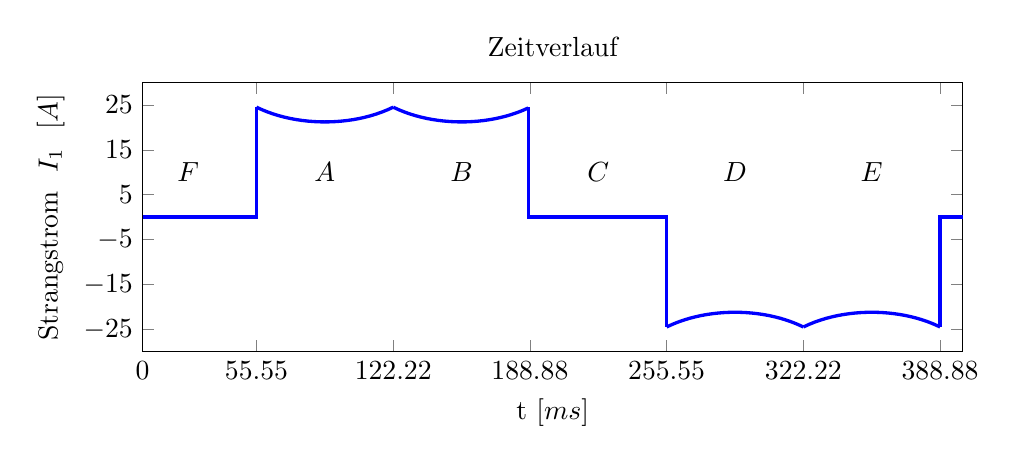
\begin{tikzpicture}
				\begin{axis}[title={Zeitverlauf},xlabel={{t} $\left [ ms \right ]$}, ylabel={{Strangstrom } $I_1$ { }$\left [ A \right ]$ },
					xtick= {0,55.55,122.22,188.88,255.55,322.22,388.88},width=12cm,height=5cm,
					xmin = 0,xmax = 400,
					ytick= {-25,-15,...,25},
					ymin = -30 , ymax = 30]
					\addplot [blue,no marks,very thick ]coordinates {(0,0) (55.55 , 0) (55.55,24.494) };%F
					\addplot [blue,no marks,very thick, domain=55.55:122.22 ] {21.213 / (sin(0.9*(x+11.11)) )}; %A
					\addplot [blue,no marks,very thick, domain=122.22:188.055 ] {21.213 / (sin(0.9*(x-55.55)) )};%B
					\addplot [blue,no marks,very thick ]coordinates {(188.055,24.494) (188.055 , 0) (255.55, 0) (255.55,-24.494) };%C
					\addplot [blue,no marks,very thick, domain=255.55:322.22 ] {21.213 / (sin(0.9*(x-388.88)) )};%D
					\addplot [blue,no marks,very thick, domain=322.22:388.88] {21.213 / (sin(0.9*(x-455.55)) )};%E
					\addplot [blue,no marks,very thick ]coordinates {(388.88,-24.494) (388.88 , 0) (400, 0)};%F
					\node[] at (axis cs:22.21,10) {$F$};
					\node[] at (axis cs:88.88,10) {$A$};
					\node[] at (axis cs:155.55,10) {$B$};
					\node[] at (axis cs:222.21,10) {$C$};
					\node[] at (axis cs:288.88,10) {$D$};
					\node[] at (axis cs:355.55,10) {$E$};
				\end{axis}
			\end{tikzpicture}
			\label{fig:20160615lsg14}
		\end{figure}
	\end{compactenum}
\end{solution}